\documentclass[xcolor ={table,usenames,dvipsnames}]{beamer}
\usepackage[italian]{babel}
\usepackage{listings}
\PassOptionsToPackage{dvipsnames}{xcolor}
\title{Risk Assessment}

\author{Authors: Tommaso Puccetti, Edoardo Dini}
\institute{Universit\`a  degli studi di Firenze}
\date{22/09/2018}
\usepackage{sansmathaccent}
\usetheme{Berlin} 
\useinnertheme{rounded}
\useoutertheme{miniframes} 
\setbeamercovered{dynamic}
 
\theoremstyle{definition}
\newtheorem{definizione}{Definizione}





\begin{document}
	
	\begin{frame}
		\maketitle
	\end{frame}
	
	\begin{frame}
		\frametitle{IT Security Management: overview (1)}
	\textbf{	Is the formal process of answering the questions:}
		\begin{figure}[h!]
			\centering
			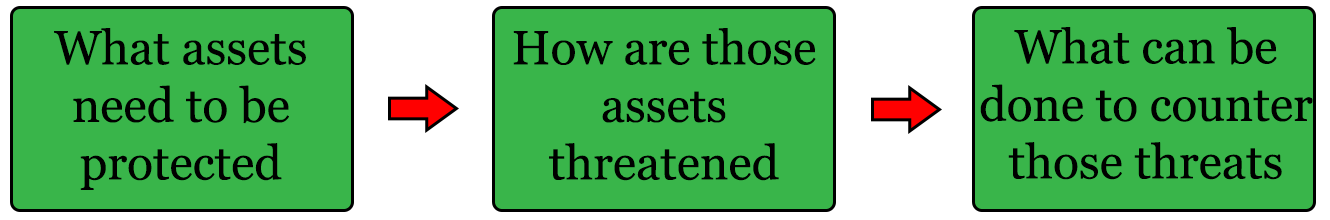
\includegraphics[scale=0.20]{img/img_01.PNG}
			\label{Interfacce di un CS}
		\end{figure}
		\begin{itemize}
			\item Ensure that asset are sufficiently protected in a cost-effective manner;
			\item Security risk assessment is needed for each asset in the organization;  that require protection;
			\item Provide the information necessary to decide what management, operational and technical controls are needed to reduce the risk identified
		\end{itemize}
	\end{frame}

	\begin{frame}
		\frametitle{IT Security Management: overview (2)}
		\begin{alertblock}{Definition:}
			 A process used to achieve and maintain appropriate levels of confidentiality, integrity, availability, accountability, authenticity, and reliability. 
		\end{alertblock}
		\begin{itemize}
			\item determining organizational IT security objectives, strategies, and policies
			\item determining organizational IT security requirements
			\item identifying and analyzing security threats to IT assets 
			\item identifying and analyzing risks
			\item specifying appropriate safeguards
			\item monitoring the implementation and operation of safeguards
			\item developing and implementing a security awareness program
			\item detecting and reacting to incidents
		\end{itemize}	
	\end{frame}

	\begin{frame}
		\frametitle{IT Security Management: a cyclic process (1)}
	    \textbf{It is important to emphasize that:}
	    \begin{itemize}
	    	\item IT security management needs to be a key part of an organization’s overall management plan.
	    	\item IT security risk assessment process should be incorporated into the
	    	wider risk assessment of all the organization’s assets and business processes.
	    	\item IT security management is a cyclic process \textbf{that must be repeated constantly} (as specified in [ISO27001]).
	    \end{itemize} 
	\end{frame}
	
	\begin{frame}
		\frametitle{IT Security Management: a cyclic process (2)}
			\begin{figure}[h!]
			\centering
			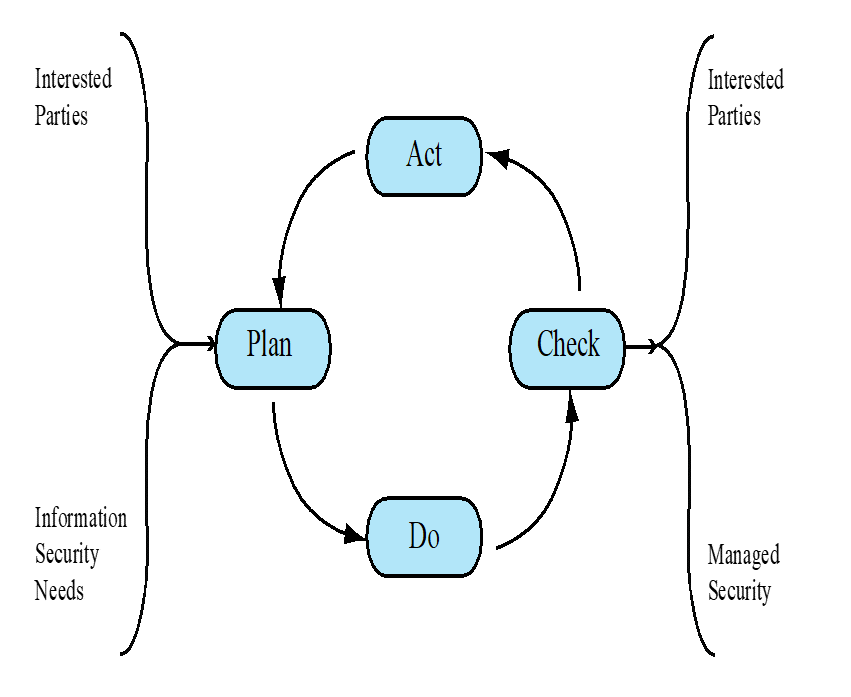
\includegraphics[scale=0.50]{img/img_02.PNG}
			\label{Interfacce di un CS}
		\end{figure}
	\end{frame}
	
	\begin{frame}
		\frametitle{IT Security Management: a cyclic process (3)}
			\begin{figure}[h!]
			\centering
			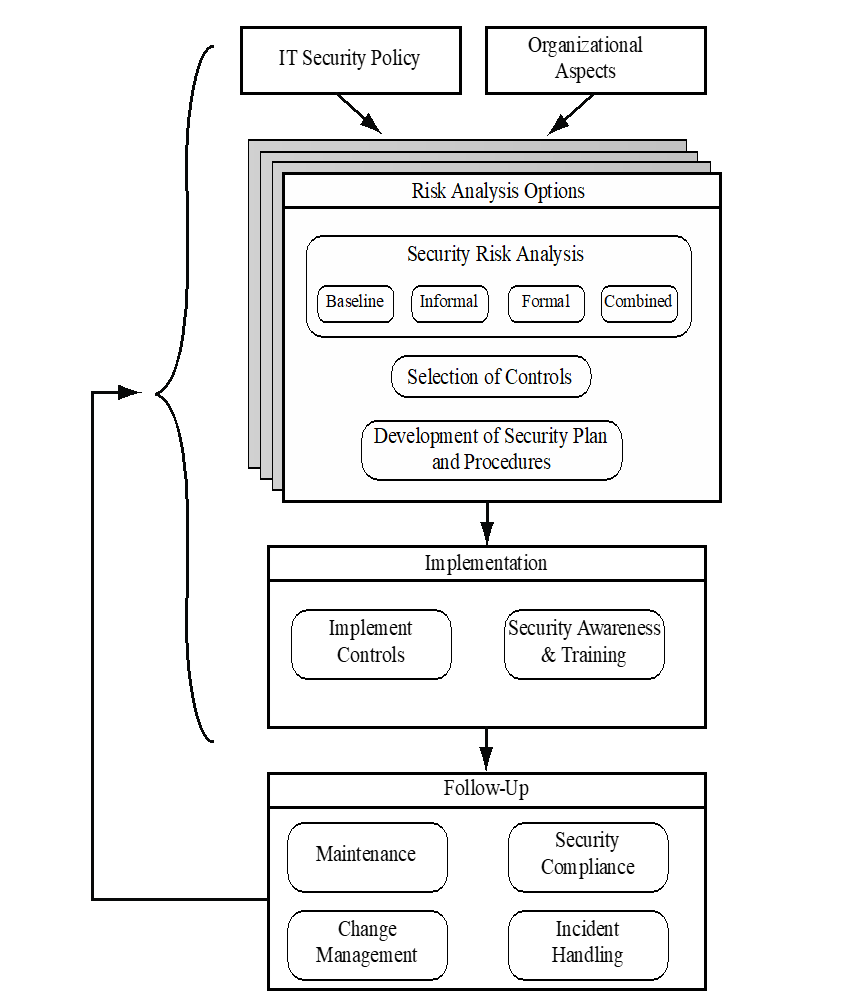
\includegraphics[scale=0.40]{img/img_03.PNG}
			\label{Interfacce di un CS}
		\end{figure}
	\end{frame}
	
	\begin{frame}
		\frametitle{Evolution and consensus}
		The discipline of IT security management has evolved considerably over the last few decades. This has occurred in response to the rapid growth of, and dependence on networked computer systems and the associated rise in risks to these systems. In the last	decade a number of national and international standards have been published. These represent a consensus on the best practice in the field. The International Standards Organization (ISO) has revised and consolidated a number of these standards into the 27000 series.
	\end{frame}

	\begin{frame}
		\frametitle{ISO 27000 series of Standards on IT Security Techniques }
		\begin{table}[]
			\resizebox{11.5cm}{!}{
				\begin{tabular}{|
					>{\columncolor[HTML]{32CB00}}l |l|}
				\hline
				27000:2012 & \begin{tabular}[c]{@{}l@{}}“Information security management systems—Overview and vocabulary” provides an\\ ­overview of information security management systems, and defines the vocabulary and\\ ­definitions used in the 27000 family of standards.\end{tabular}              \\ \hline
				27001:2005 & \begin{tabular}[c]{@{}l@{}}“Information security management systems—Requirements” specifies the requirements for\\ establishing, implementing, operating, monitoring, reviewing, maintaining, and improving a\\ documented Information Security Management System.\end{tabular} \\ \hline
				27002:2005 & \begin{tabular}[c]{@{}l@{}}“Code of practice for information security management” provides guidelines for informa-\\ tion security management in an organization and contains a list of best-practice security\\ controls. It was formerly known as ISO17799.\end{tabular}      \\ \hline
				27003:2010 & \begin{tabular}[c]{@{}l@{}}“Information security management system implementation guidance” details the process\\ from inception to the production of implementation plans of an Information Security\\ Management System specification and design.\end{tabular}                \\ \hline
				27004:2009 & \begin{tabular}[c]{@{}l@{}}“Information security management—Measurement” provides guidance to help organiza-\\ tions measure and report on the effectiveness of their Information Security Management\\ System processes and controls.\end{tabular}                             \\ \hline
				27005:2011 & \begin{tabular}[c]{@{}l@{}}“Information security risk management” provides guidelines on the information security\\ risk management process. It supersedes ISO13335-3/4.\end{tabular}                                                                                           \\ \hline
				27006:2007 & \begin{tabular}[c]{@{}l@{}}“Requirements for bodies providing audit and certification of information security\\ ­management systems” specifies requirements and provides guidance for these bodies.\end{tabular}                                                                \\ \hline
			\end{tabular}
		}
		\end{table}
	\end{frame}

	\begin{frame}
		\frametitle{Organizational Context and Security Policy}
		\begin{figure}[h!]
			\centering
			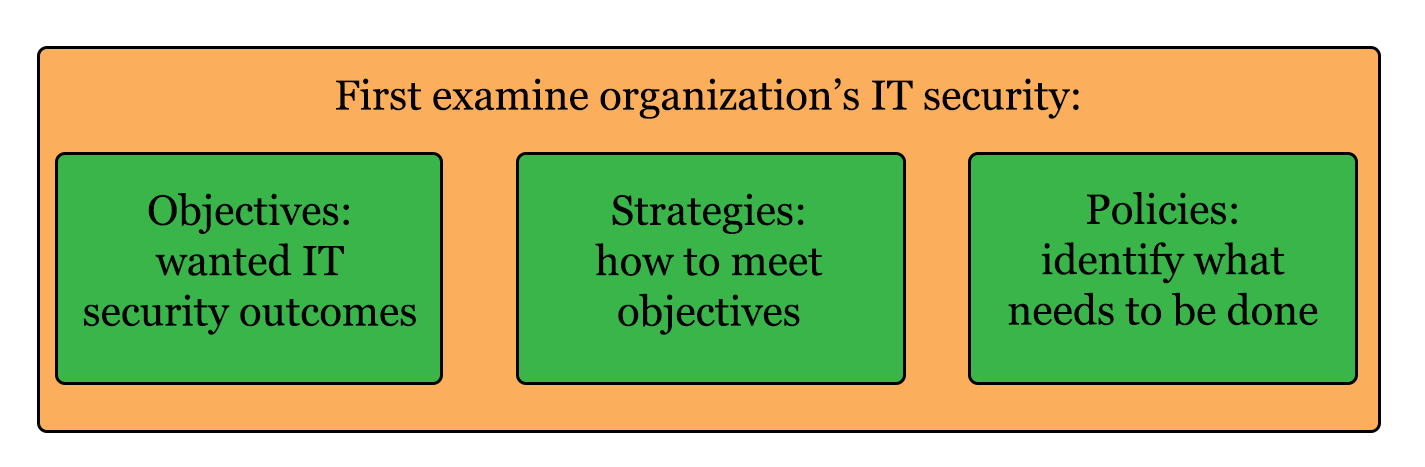
\includegraphics[scale=0.20]{img/img_04.PNG}
			\label{Interfacce di un CS}
		\end{figure}
		In IT security management process comprises an examination of the organization's IT security \textbf{object, strategies and policies}. This can only occur in the wider context of the organization's management.
	
	\end{frame}

	\begin{frame}
		\frametitle{Security Objectives}
		\begin{itemize}
			\item What key aspects of the organization require IT support in order to function efficiently?
			\item What tasks can only be performed with IT support?
			\item Which essential decisions depend on the accuracy, currency, integrity, or availability of data managed by the IT systems?
			\item What data created, managed, processed, and stored by the IT systems need
			protection?
			\item What are the consequences to the organization of a security failure in their IT systems?
		\end{itemize}
	\end{frame}

	\begin{frame}
		\frametitle{Security Strategy}
		Once the objectives are listed, some broad strategy statements can be developed.
		These outline in general terms how the identified objectives will be met in a ­consistent manner across the organization:
		\begin{itemize}
			 \item The topics and details in the strategy ­statements
			depend on the identified objectives, the size of the organization, and the importance of the IT systems to the organization. 
			\item The strategy statements should address the approaches the organization will use to manage the security of its IT systems. Given the organizational security objectives and strategies, an organizational
		\end{itemize}	
	\end{frame}

	\begin{frame}
		\frametitle{Security Policy}
		Given the organizational security objectives and strategies, an organizational
		security policy is developed that describes what the objectives and strategies are and the process used to achieve them. 
		
		INSERIRE ELENCO PUNTATO
	\end{frame}

	\begin{frame}
		\frametitle{Management Support }
		IT security policy must be supported by senior management
		Need IT security officer
		\begin{itemize}
			\item To provide consistent overall supervision
			\item Liaison with senior management
			\item Maintenance of IT security objectives, strategies, policies
			\item Handle incidents
			\item Management of IT security awareness and training programs
			\item Interaction with IT project security officers
		\end{itemize}
		Large organizations need separate IT project security officers associated with major projects and systems
	\end{frame}

	\begin{frame}
		\frametitle{Security Risk Assessment}
		\begin{figure}[h!]
			\centering
			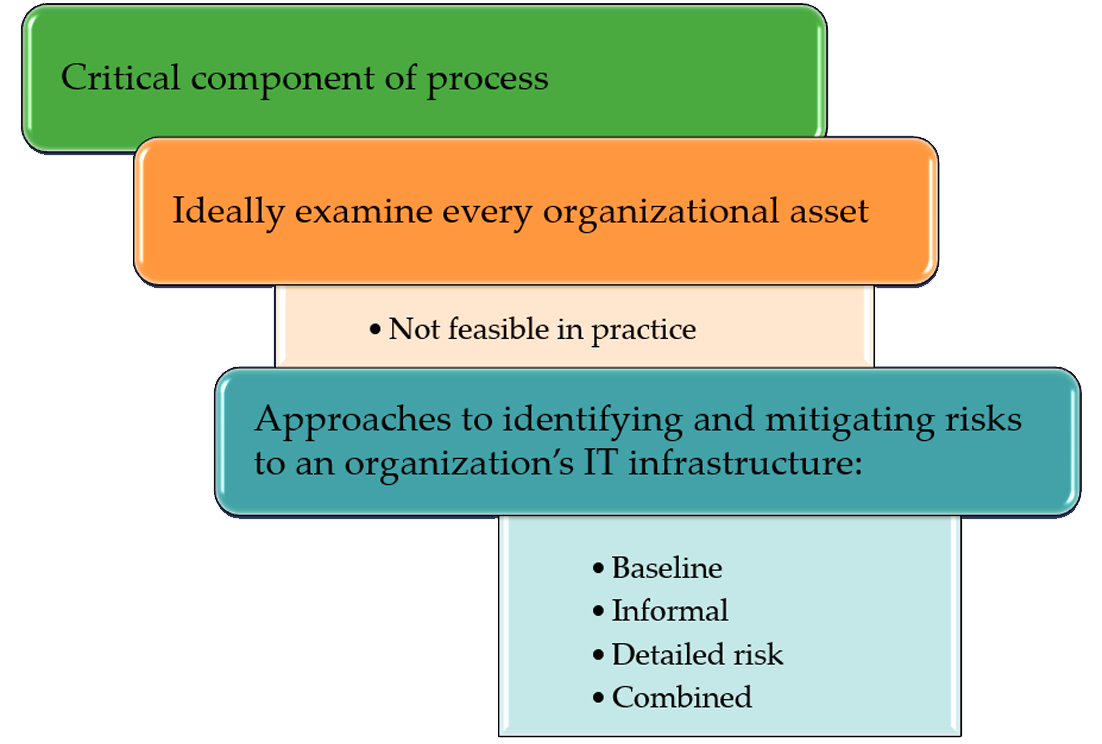
\includegraphics[scale=0.25]{img/img_05.PNG}
			\label{Interfacce di un CS}
		\end{figure}
	\end{frame}

		
	\begin{frame}
		\frametitle{Baseline Approach}
			\begin{figure}[h!]
				\centering
				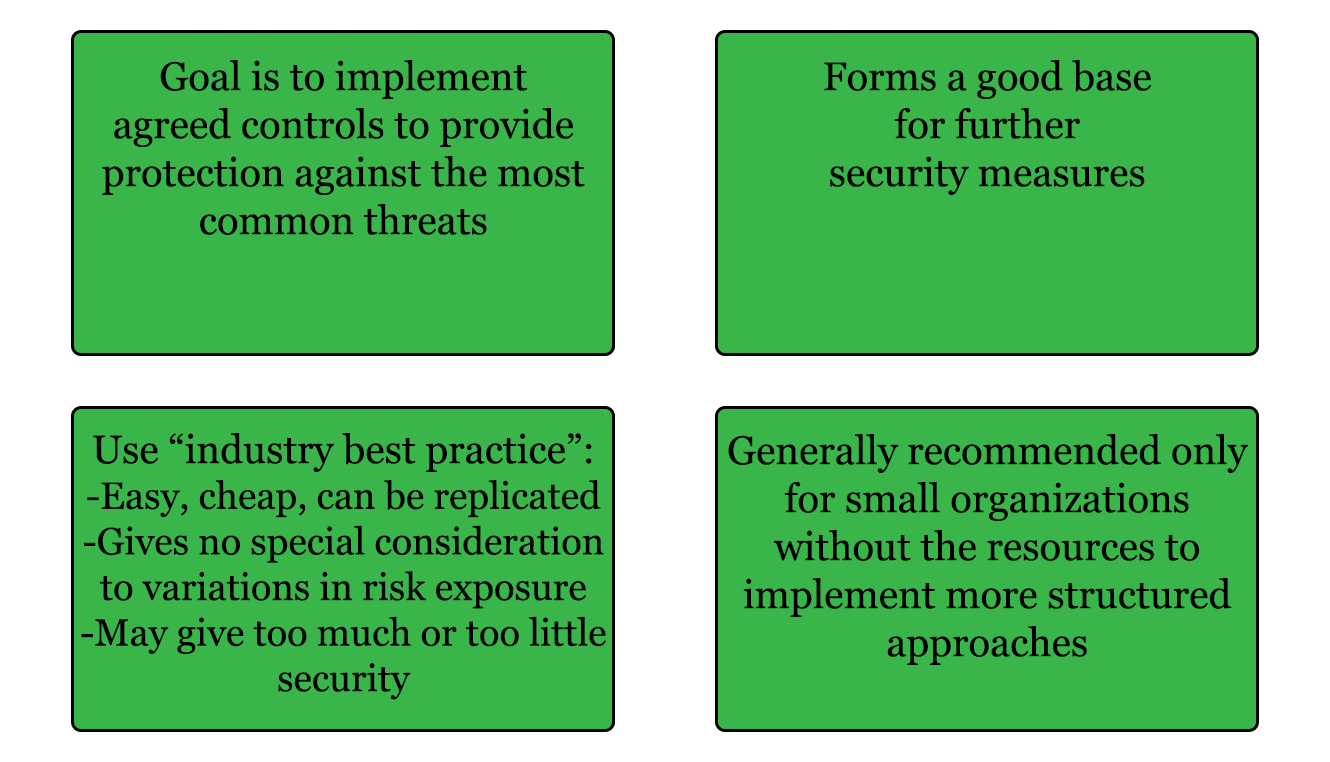
\includegraphics[scale=0.23]{img/img_06.PNG}
				\label{Interfacce di un CS}
			\end{figure}
			%\begin{itemize} 
			%	\item Goal is to implement agreed controls to provide protection against the most common threats
			%	\item Forms a good base for further security measures
			%	\item Use “industry best practice”
			%	\begin{itemize}
			%		\item Easy, cheap, can be replicated
			%		\item Gives no special consideration to variations in risk exposure
			%		\item May give too much or too little security
			%	\end{itemize}
			%	\item Generally recommended only for small organizations without the resources to implement more structured approaches
			%\end{itemize}
	\end{frame}
	
	\begin{frame}
		\frametitle{Informal Approach}
		\begin{figure}[h!]
			\centering
			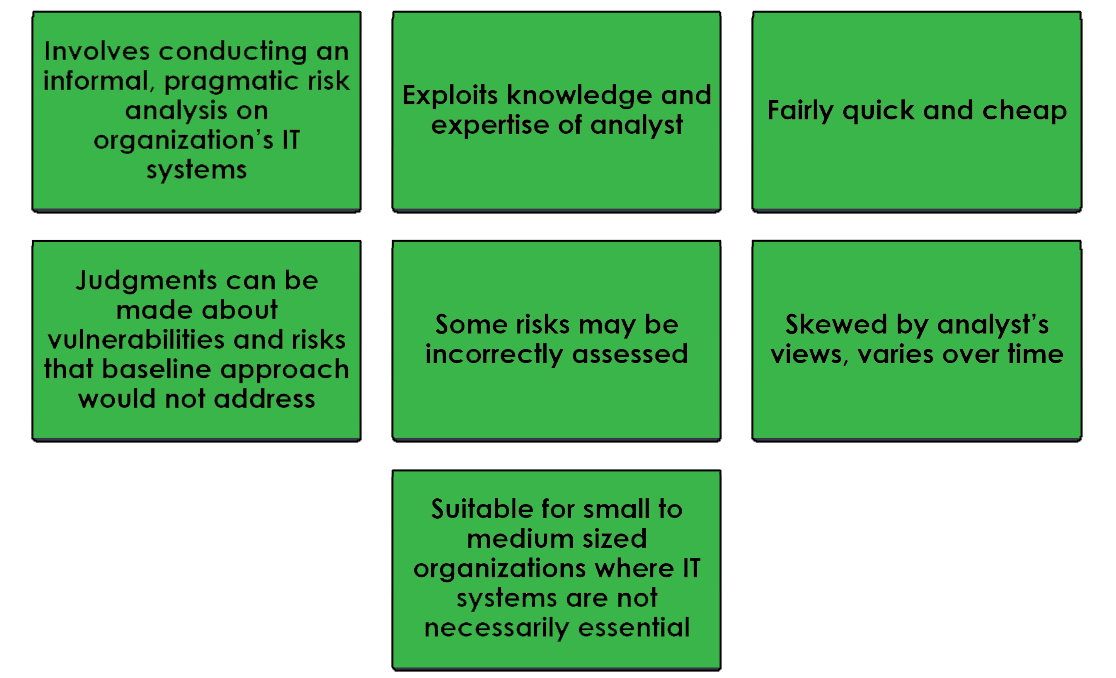
\includegraphics[scale=0.27]{img/img_07.PNG}
			\label{Interfacce di un CS}
		\end{figure}
	\end{frame}

	\begin{frame}
		\frametitle{Detailed Risk Analysis}
		\begin{figure}[h!]
			\centering
			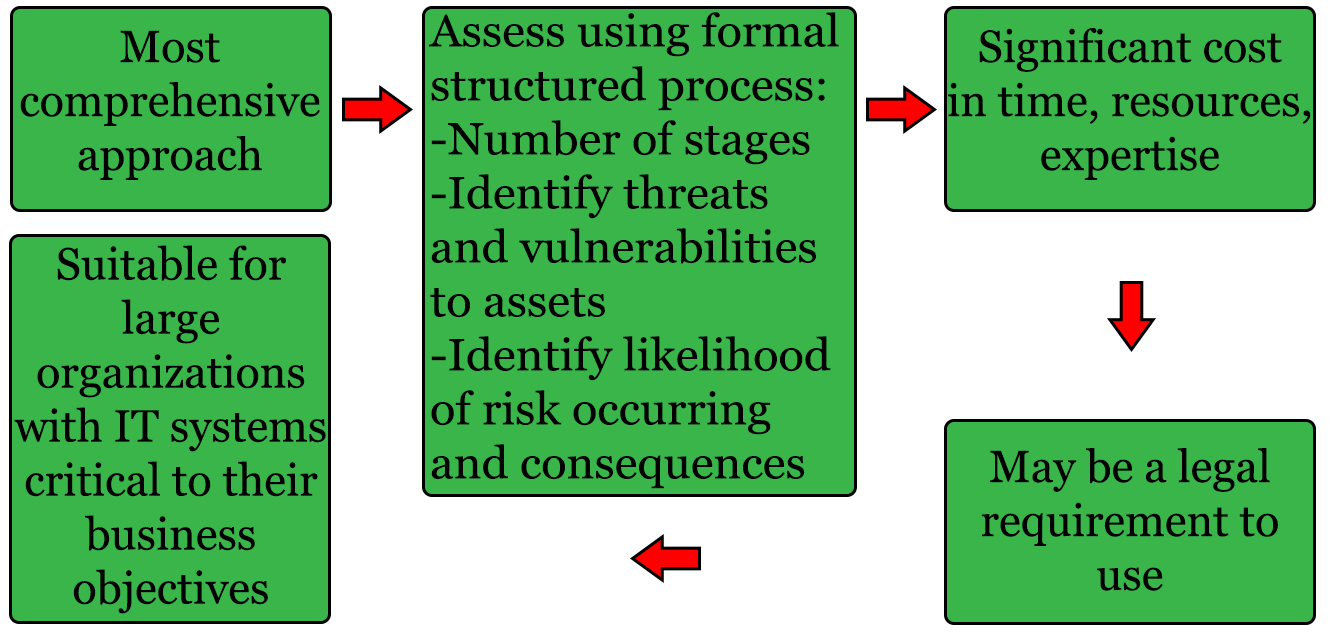
\includegraphics[scale=0.23]{img/img_08.PNG}
			\label{Interfacce di un CS}
		\end{figure}
	\end{frame}

	\begin{frame}
		\frametitle{Combined Approach (1)}
		IMMAGINE 
		 Aim is to provide reasonable levels of protection as quickly as possible then to examine and adjust the protection controls deployed on key systems over time:
		Over time, this can result in the most appropriate and cost-effective security controls being selected and implemented on these systems
	\end{frame}
	
	\begin{frame}
		\frametitle{Combined Approach (2)}
		\begin{enumerate}
			\item Approach starts with the implementation of suitable baseline security recommendations on all systems
			\item Next, systems either exposed to high risk levels or critical to the organization's business objectives are identified in the high-level risk assessment
			\item A decision can then be made to possibly conduct an immediate informal risk assessment on key systems, with the aim of relatively quickly tailoring controls to more accurately reflect their requirements
			\item Lastly, an ordered process of performing detailed risk analyses of these systems can be instituted
		\end{enumerate}
	\end{frame}

	\begin{frame}
		\frametitle{Detailed Security Risk Analysis (1)}
		\begin{figure}[h!]
			\centering
			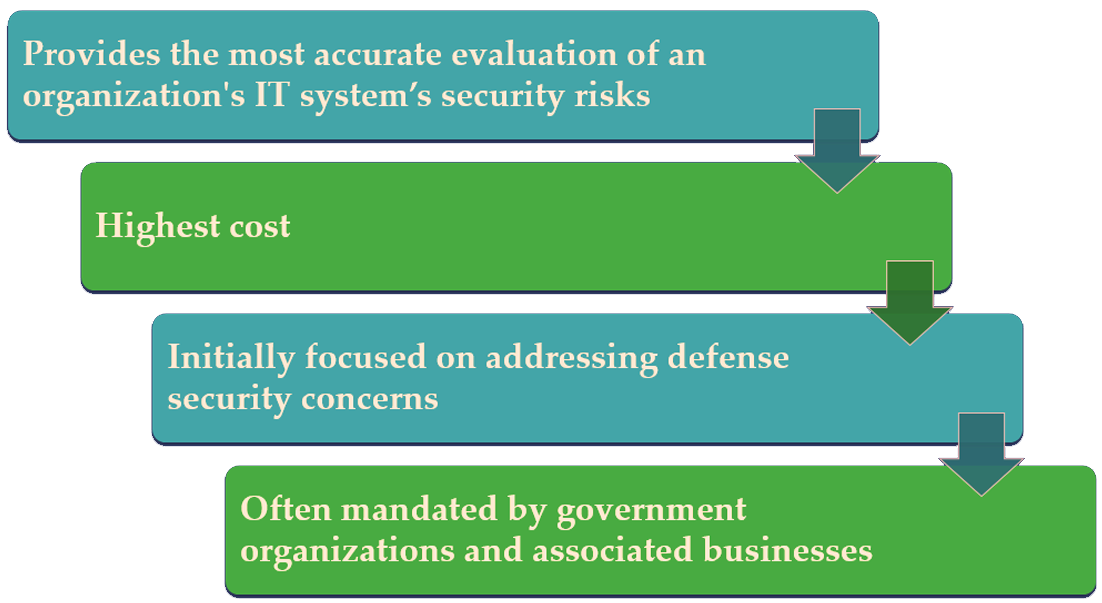
\includegraphics[scale=0.27]{img/img_09.PNG}
			\label{Interfacce di un CS}
		\end{figure}
		\end{frame}
	
	\begin{frame}
		\frametitle{Detailed Security Risk Analysis (2)}
		\begin{figure}[h!]
			\centering
			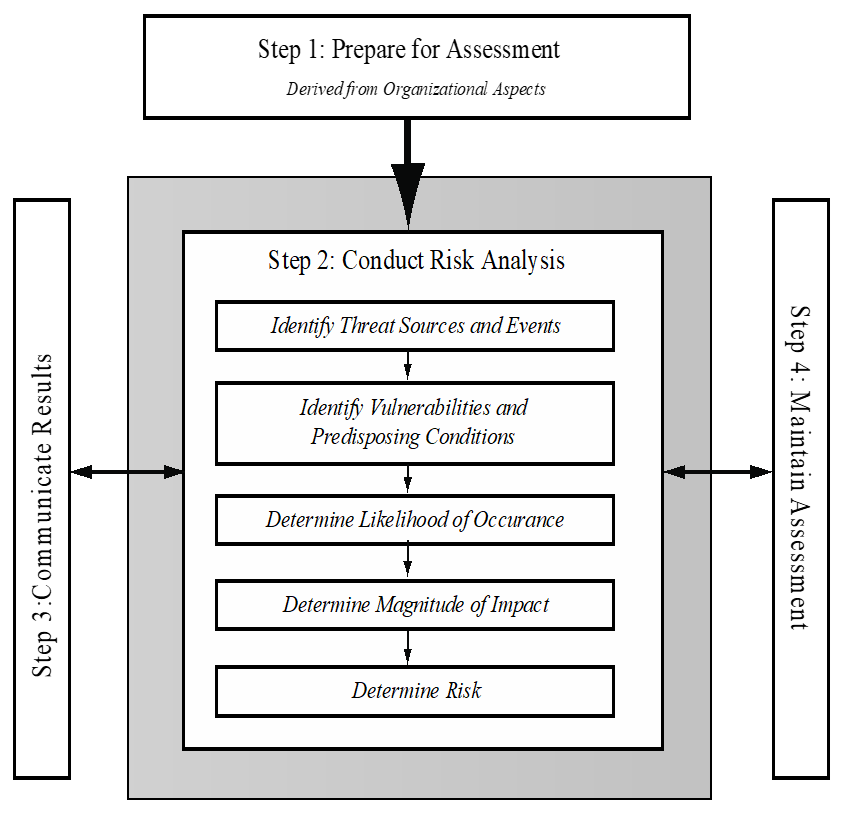
\includegraphics[scale=0.47]{img/img_10.PNG}
			\label{Interfacce di un CS}
		\end{figure}
	\end{frame}

	\begin{frame}
		\frametitle{Establishing the Context (1)}
		\begin{itemize}
			\item	Initial steps 
			\begin{itemize}
				\item Determine the basic parameters of the risk assessment
				\item Identify the assets to be examined
			\end{itemize}
			\item Explores political and social environment in which the organization operates \begin{itemize}
				\item 	Legal and regulatory constraints
				\item	Provide baseline for organization’s risk exposure
			\end{itemize}
			\item The \textbf{risk appetite} is the level of risk the organization views as acceptable
		\end{itemize}	
	\end{frame}

	\begin{frame}
		\frametitle{Establishing the Context (2)}
		\begin{figure}[h!]
			\centering
			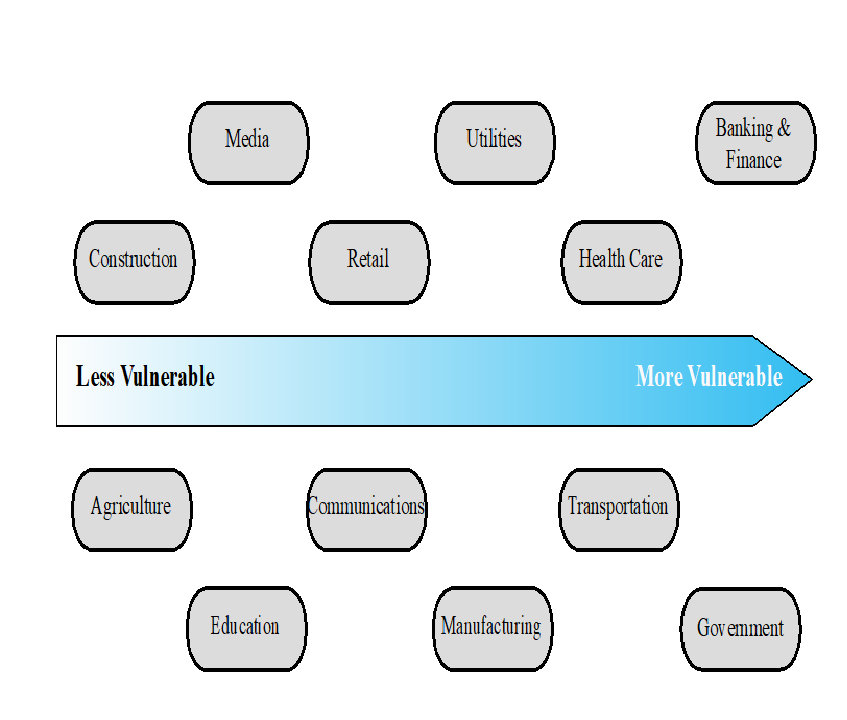
\includegraphics[scale=0.45]{img/img_11.PNG}
			\label{Interfacce di un CS}
		\end{figure}
	\end{frame}

	\begin{frame}
		\frametitle{Terminology}
			\begin{itemize}
				\item \textbf{Asset}: a system resource or capability of value to its owner that requires protection. 
				\item \textbf{Threat}: a potential for a threat source to exploit a vulnerability in some asset, which if it occurs may compromise the security of the asset and cause harm to the asset’s owner
				\item \textbf{Vulnerability}: a flaw or weakness in an asset’s design, implementation, or operation and management that could be exploited 		by some threat
				\item \textbf{Risk}: The potential for loss computed as the 	combination of the likelihood that a given threat exploits some vulnerability to an asset, and the magnitude of harmful consequence that results to the asset’s owner.
			\end{itemize}
	\end{frame}

	\begin{frame}
		\frametitle{Asset Identification}
		\textit{\textbf{"What assets we need to protect?"}}
		\begin{itemize}
			\item These assets need to be identified and their value to the organization assessed.
			\item The ideal is to consider every conceivable asset, in practice this is not possible. Rather the goal here is to identify all assets that contribute significantly to attaining the organization’s objectives and whose compromise the organization’s operation. 
			\item A security experts may not have an high knowledge of the organization's oepration and structure, so experts for each area of the organization are needed for the process.
		\end{itemize}
	\end{frame}

	\begin{frame}
		\frametitle{Threat Identification (1)}
		\textbf{\textit{"Who or what could cause harm to the assets?"}}
		\begin{itemize}
			\item Identifying possible threats and threat sources requires the use of a \textbf{variety of sources}, along with the experience of the risk assessor. 
			\item  Organization’s define threat scenarios to describe how the tactics, techniques, and procedures employed by an attacker can contribute to, or cause, harm. 
		\end{itemize}
		
		
	\end{frame}

	\begin{frame}
		\frametitle{Threat Identification (2)}
		\begin{enumerate}
			\item  \textbf{Motivation}: Why would they target this organization; how motivated are they?
			\item \textbf{Capability}: What is their level of skill in exploiting the threat?
			\item \textbf{Resources}: How much time, money, and other resources could they deploy?
			\item \textbf{Probability of attack}: How likely and how often would your assets be targeted?
			\item \textbf{Deterrence}: What are the consequences to the attacker of being identified?	
		\end{enumerate}
	\end{frame}
	
	\begin{frame}
		\frametitle{Vulnerability Identification}
		\begin{itemize}
			\item Identify exploitable flaws or weaknesses in organization’s IT systems or processes
			\begin{itemize}
				\item Determines applicability and significance of threat to organization
			\end{itemize}
			\item Need combination of threat and vulnerability to create a risk to an asset
			\item utcome should be a list of threats and vulnerabilities with brief descriptions of how and why they might occur
		\end{itemize}
	\end{frame}

	\begin{frame}
		\frametitle{Analyze Risks}
		\begin{itemize}
			\item Specify likelihood of occurrence of each identified threat to asset given existing controls
			\item Specify consequence should threat occur
			\item Hard to determine accurate               probabilities and realistic cost          consequences
			\item Use qualitative, not quantitative, ratings 
			\item Derive overall risk rating for each threat
		\end{itemize}
		\begin{alertblock}{Definition:}
			\textbf{Risk = probability threat occurs x cost to organization}
		\end{alertblock}
	\end{frame}

	





	

	
\end{document}
